\documentclass{beamer}

\usepackage[utf8]{inputenc}
\usepackage{hyperref}

\usetheme{Berkeley}
\beamertemplatenavigationsymbolsempty
\setbeamertemplate{headline}{}
 
\title{Erfassen von Daten in FoodChain-Lab}
\date{}
 
\begin{document}
\maketitle

\section{Aufgaben}
\begin{frame}
	\begin{itemize}
		\item Importieren Sie folgende Datei in eine leere Datenbank: \url{https://github.com/SiLeBAT/BfROpenLabResources/raw/master/GitHubPages/documents/1_Lieferliste Caterer 1a.xlsx}
		\item Generieren Sie ein neues Template zur Dateneingabe für fehlende Daten.
        \item Füllen Sie das Template.
        \item Importieren Sie die neuen Daten in die Datenbank.
	\end{itemize}
\end{frame}
 
\section{1}
\begin{frame}
	\begin{center}
  		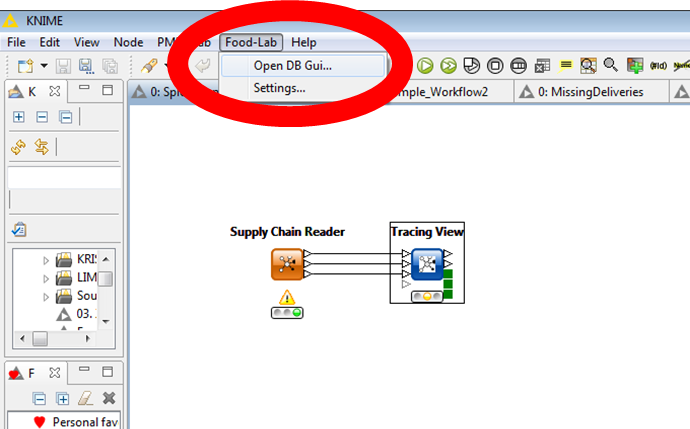
\includegraphics[height=0.6\textheight]{1.png}
	\end{center}
	\begin{itemize}
		\item Öffnen Sie das Datenbankfenster über das Menü in \textbf{KNIME} via \textbf{Food-Lab $>$ Open DB Gui...}.
	\end{itemize}
\end{frame}

\section{2}
\begin{frame}
	\begin{center}
  		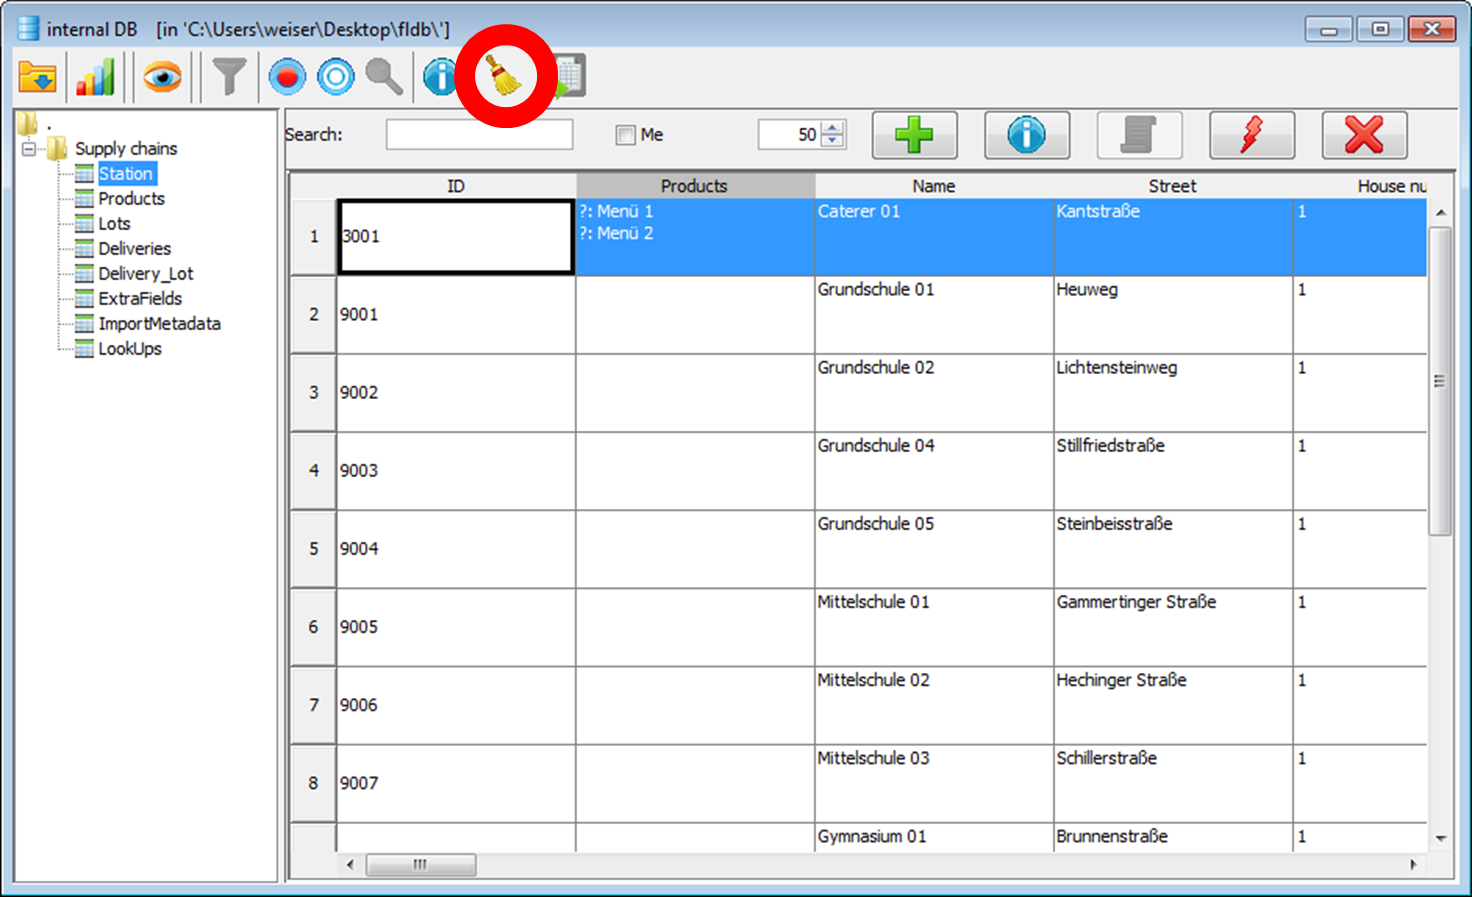
\includegraphics[height=0.6\textheight]{2.png}
	\end{center}
	\begin{itemize}
		\item Das Datenbankfenster öffnet sich.
		\item Drücken Sie auf das Symbol mit dem Besen in der Toolbar des Fensters. Das bewirkt einen Reset der Datenbank. Achtung: Alle Daten in der lokalen Datenbank werden dadurch gelöscht! Eine neue leere Datenbank wird erstellt.
		\item Sie können durch Drücken auf den roten Knopf in der Toolbar vorher eine Sicherung der aktuellen Datenbank erstellen.
	\end{itemize}
\end{frame}

\section{3}
\begin{frame}
	\begin{center}
  		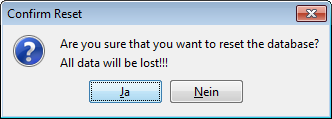
\includegraphics[height=0.3\textheight]{3.png}
	\end{center}
	\begin{itemize}
		\item Bestätigen Sie den Reset der Datenbank mit \textbf{Ja}.
	\end{itemize}
\end{frame}

\section{4}
\begin{frame}
	\begin{center}
  		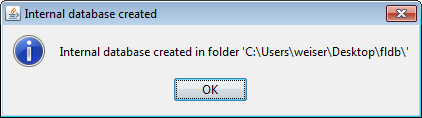
\includegraphics[width=0.9\textwidth]{4.png}
	\end{center}
	\begin{itemize}
		\item Das Datenbankfenster schließt sich, dann sollten Sie diesen Dialog sehen.
		\item Bestätigen Sie den Dialog mit \textbf{OK}. Dann öffnet sich das Datenbankfenster wieder mit leeren Tabellen.
	\end{itemize}
\end{frame}

\section{5}
\begin{frame}
	\begin{center}
  		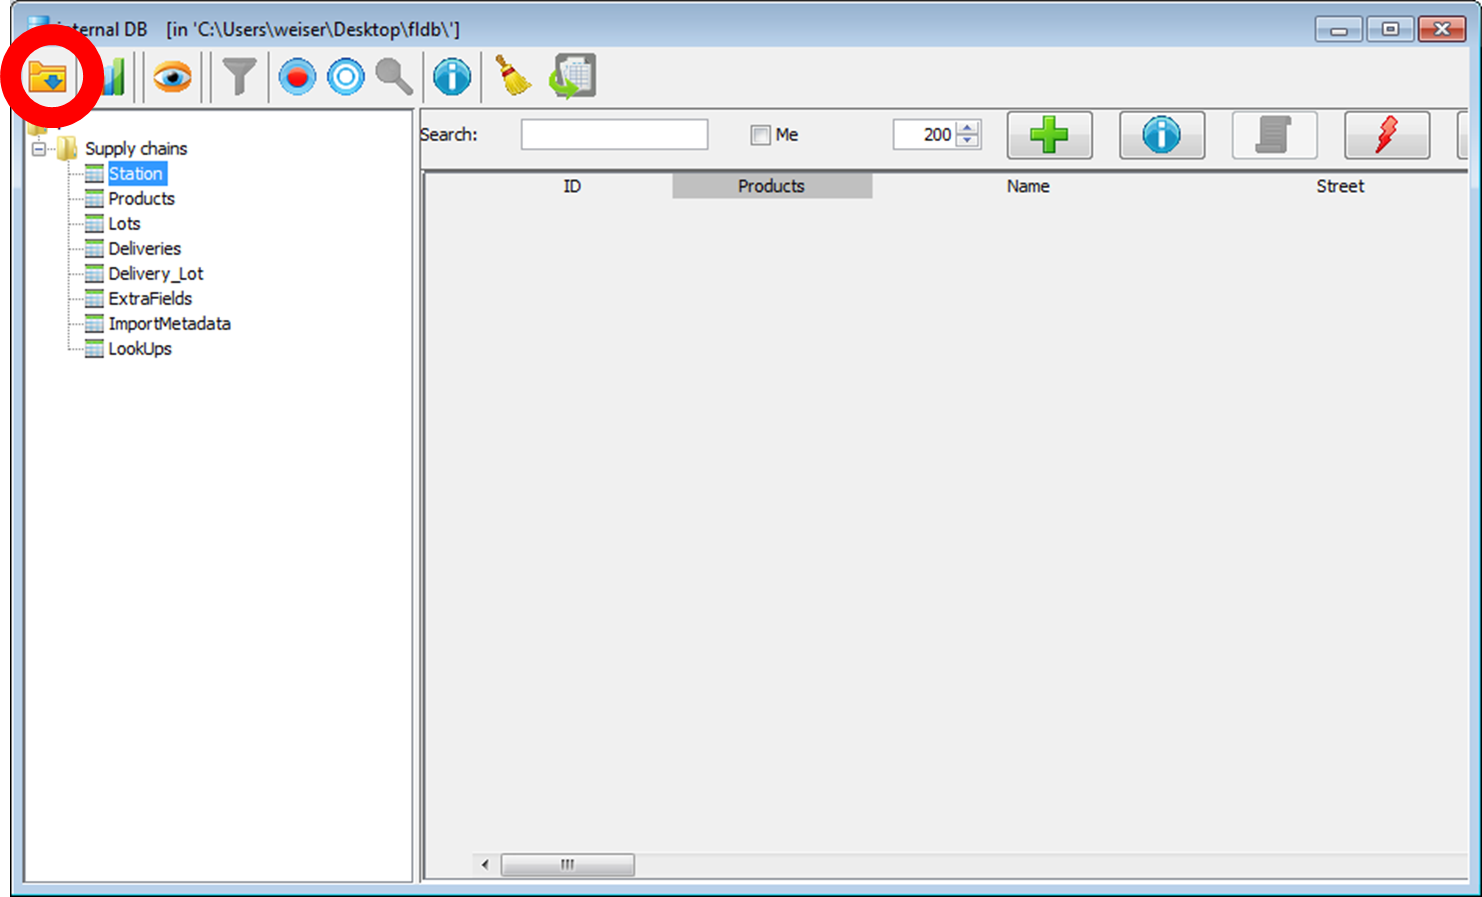
\includegraphics[width=0.9\textwidth]{5.png}
	\end{center}
	\begin{itemize}
		\item Drücken Sie auf das Ordnersymbol mit dem blauen Pfeil.
		\item Dadurch öffnet sich der Importdialog.
	\end{itemize}
\end{frame}

\section{6}
\begin{frame}
	\begin{center}
  		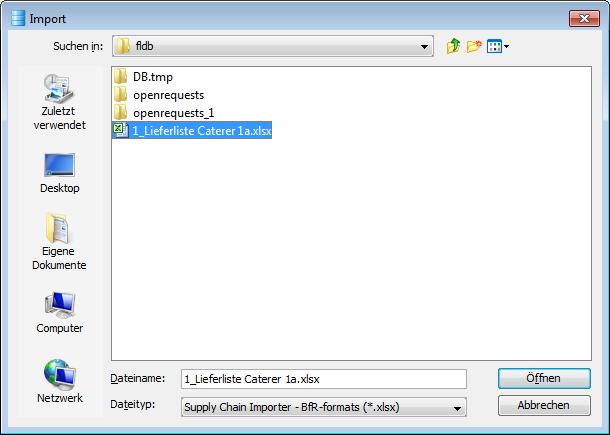
\includegraphics[height=0.6\textheight]{6.png}
	\end{center}
	\begin{itemize}
		\item Wählen Sie im Importdialog die Exceldatei aus, die Sie vorher heruntergeladen haben von  \url{https://github.com/SiLeBAT/BfROpenLabResources/raw/master/GitHubPages/documents/1_Lieferliste Caterer 1a.xlsx}
		\item Klicken Sie auf \textbf{Öffnen}.
	\end{itemize}
\end{frame}

\section{7}
\begin{frame}
	\begin{center}
  		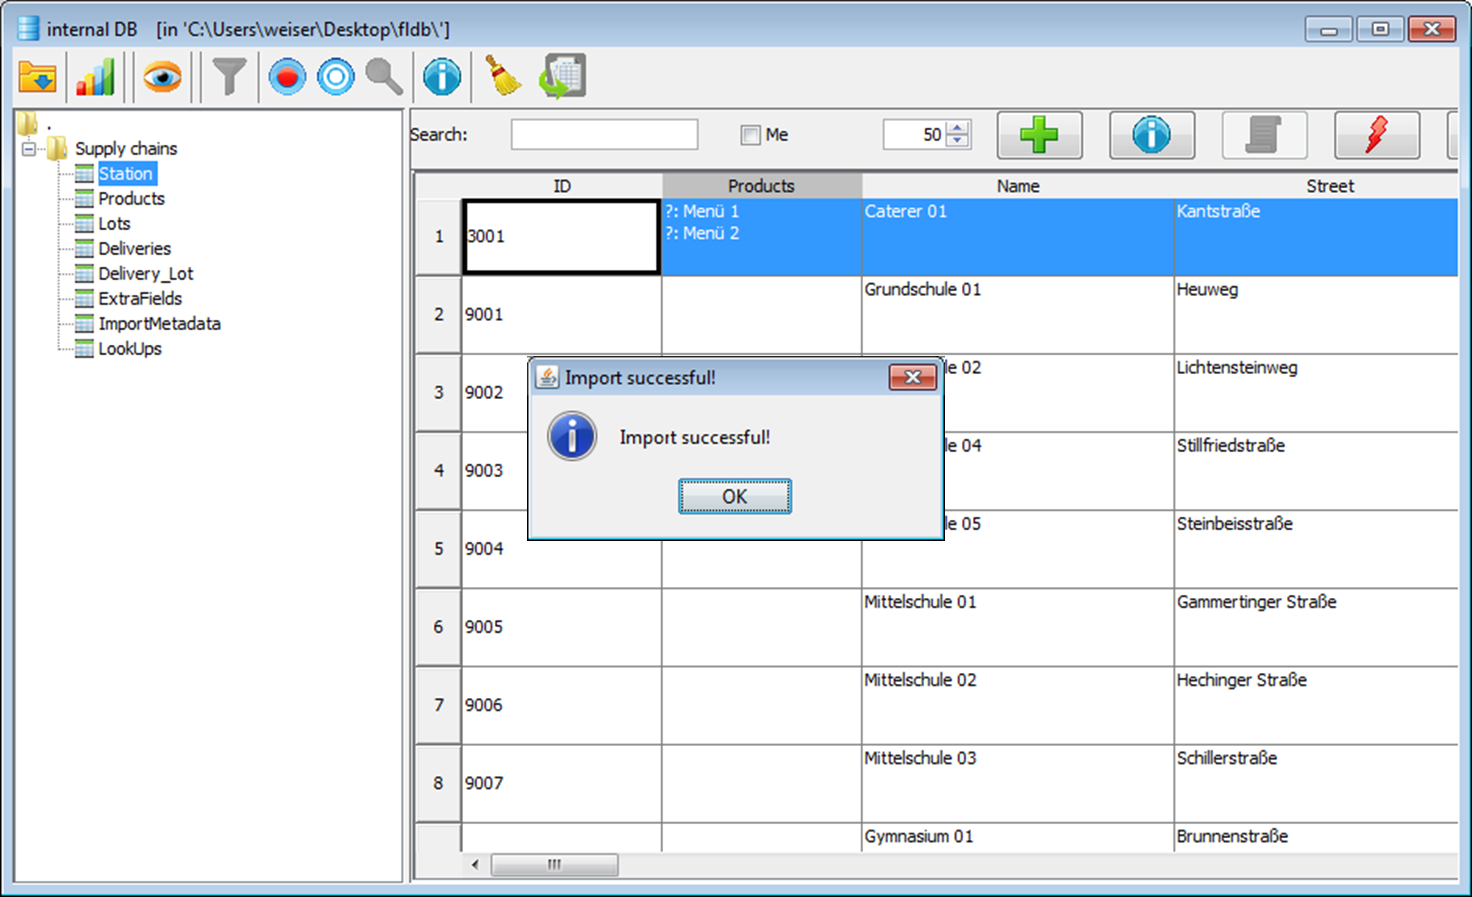
\includegraphics[height=0.6\textheight]{7.png}
	\end{center}
	\begin{itemize}
		\item Die Tabellen der Datenbank haben sich gefüllt.
		\item Der erfolgreiche Import wird durch ein kleines Fenster  bekanntgegeben.
        \item Schließen Sie dieses Fenster durch Klicken auf \textbf{OK}.
        \item Sie können sich jetzt die importierten Daten z.B. in einem TracingView anschauen, siehe ab Punkt 8 im Tutorial \url{http://foodrisklabs.bfr.bund.de/index.php/erstellen-eines-workflow-in-foodchain-lab-teil-1/} und in \url{http://foodrisklabs.bfr.bund.de/index.php/erstellen-eines-workflows-in-foodchain-lab-teil-2/}.
	\end{itemize}
\end{frame}

\section{8}
\begin{frame}
	\begin{center}
  		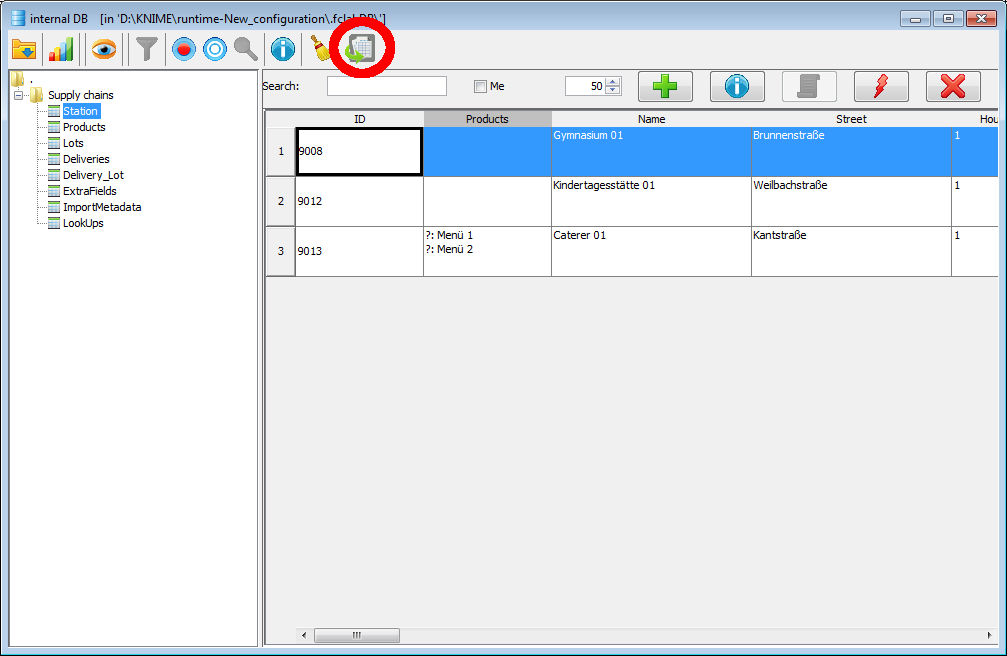
\includegraphics[width=0.7\textwidth]{8.png}
	\end{center}
	\begin{itemize}
		\item Drücken Sie nun auf das Tabellensymbol mit dem grünen Pfeil ganz rechts in der Toolbar.
	\end{itemize}
\end{frame}

\section{9}
\begin{frame}
	\begin{center}
  		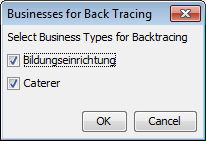
\includegraphics[height=0.5\textheight]{9.png}
	\end{center}
	\begin{itemize}
		\item Dadurch öffnet sich ein Auswahldialog, der es Ihnen ermöglicht die Betriebsarten zu definieren, für die fehlende Rückverfolgungsdaten gesammelt werden sollen.
		\item Bestätigen Sie Ihre Auswahl mit \textbf{OK}.
	\end{itemize}
\end{frame}

\section{10}
\begin{frame}
	\begin{center}
  		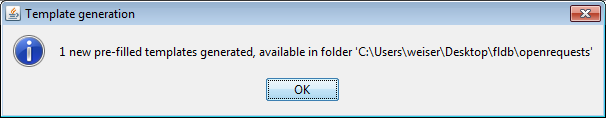
\includegraphics[height=0.2\textheight]{10.png}
	\end{center}
	\begin{itemize}
		\item Es werden nun alle fehlenden Daten ermittelt und automatisch Templates generiert, die für die Datenerfassung optimiert sind.
		\item Im folgenden Fenster wird Ihnen angezeigt, wieviele neue Templates erstellt worden sind und in welchem Ordner sich diese befinden.
		\item Merken Sie sich diesen Ordner bzw. suchen Sie diesen Ordner mit Ihrem Dateimanager auf.
		\item Klicken Sie nun \textbf{OK}.
	\end{itemize}
\end{frame}

\section{11}
\begin{frame}
	\begin{center}
  		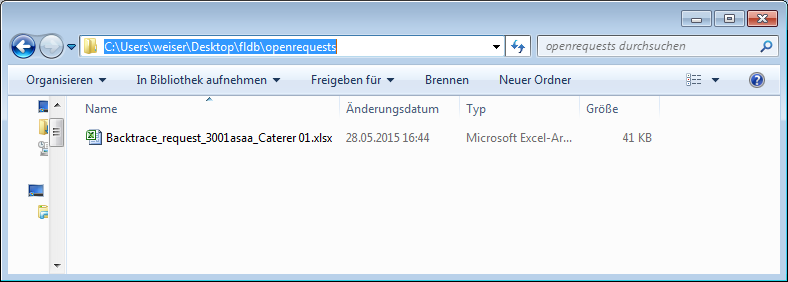
\includegraphics[height=0.4\textheight]{11.png}
	\end{center}
	\begin{itemize}
		\item Öffnen Sie das erzeugte Template durch Doppelklick in Ihrem Dateimanager.
		\item Zur Bearbeitung der Datei ist es neben Excel auch möglich auf freie Software wie z.B. LibreOffice zurückzugreifen.
	\end{itemize}
\end{frame}

\section{12}
\begin{frame}
	\begin{center}
  		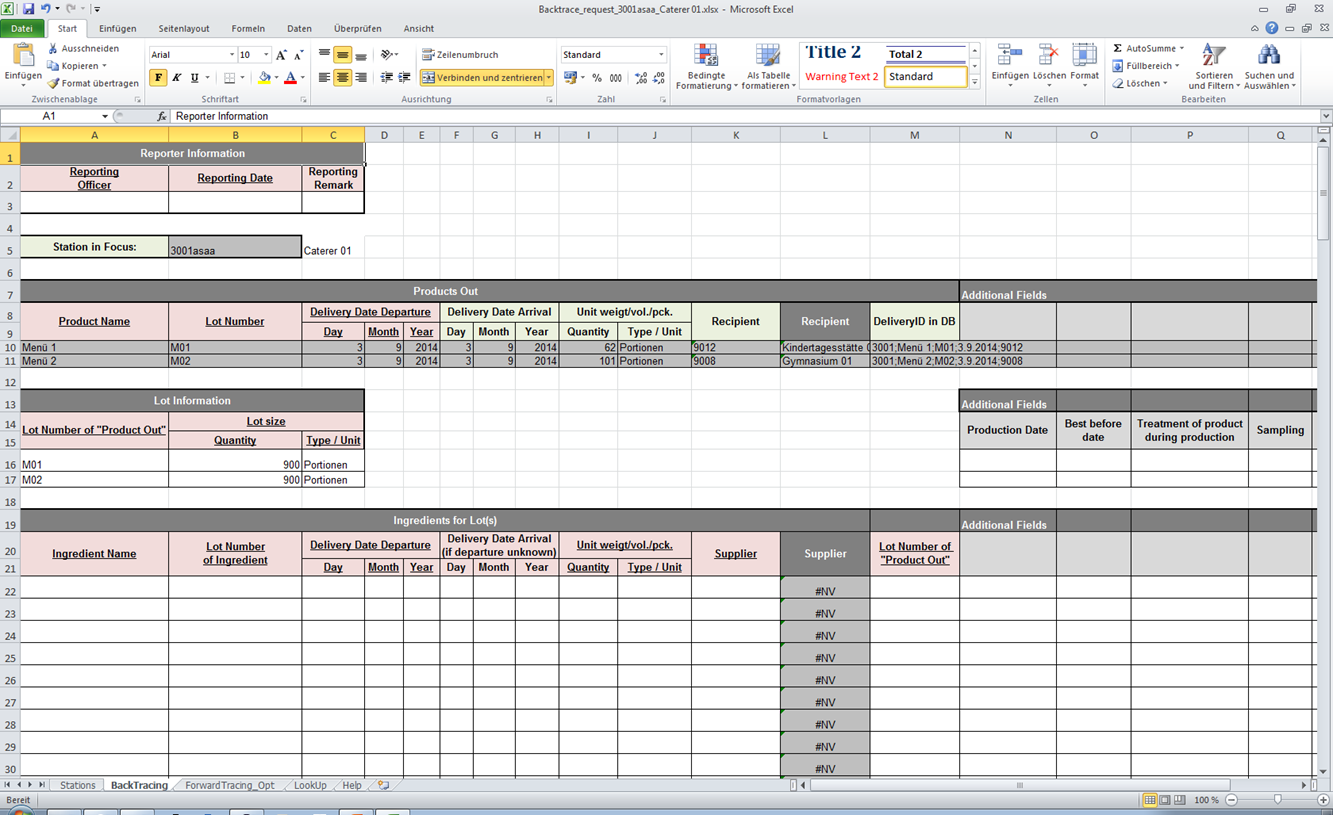
\includegraphics[height=0.5\textheight]{12.png}
	\end{center}
	\begin{itemize}
		\item Die Exceldatei besteht aus mehreren Tabellenblättern.
		\item Wesentlich sind: \textbf{Stations}, \textbf{BackTracing}, \textbf{LookUp}
		\item Das Bild zeigt das Tabellenblatt \textbf{BackTracing}, in dem bereits einige Lieferungen automatisch eingetragen worden sind.
		\item Es geht darum die zugehörigen Vorlieferungen/Zutaten zu ermitteln.
		\item Im wesentlichen müssen die Felder mit den roten Überschriften ausgefüllt/korrigiert werden.
	\end{itemize}
\end{frame}

\section{13}
\begin{frame}
	\begin{center}
  		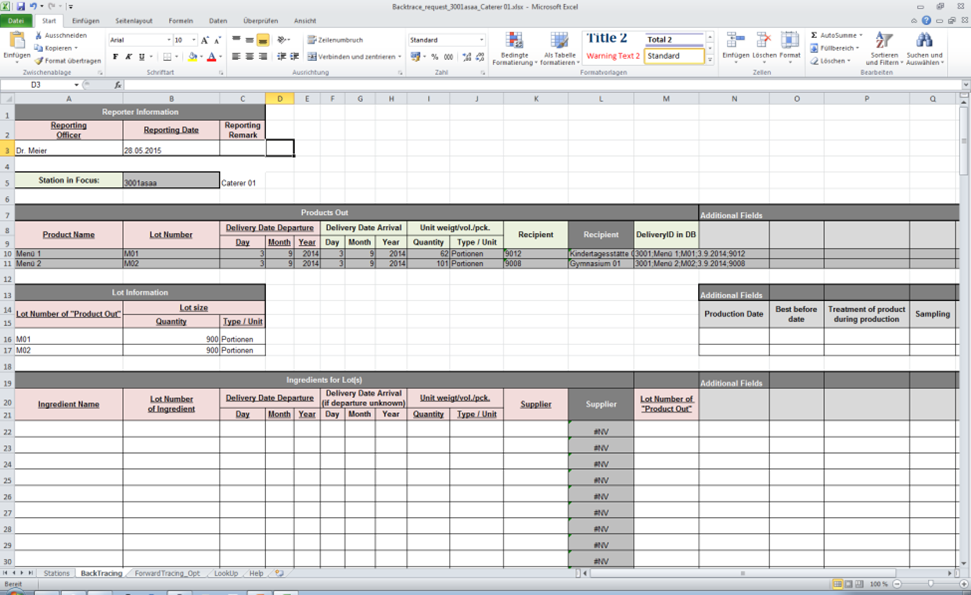
\includegraphics[height=0.65\textheight]{13.png}
	\end{center}
	\begin{itemize}
		\item Ganz oben, in der 3. Zeile müssen Informationen zum Datenerfasser gemacht werden.
		\item In Zeile 5 steht die Information, in welcher Station die Daten erfasst werden müssen.
		\item In den Zeilen 7-11 befinden sich die Lieferungen, zu denen die konkreten Zutaten gesucht werden.
	\end{itemize}
\end{frame}

\section{14}
\begin{frame}
	\begin{center}
  		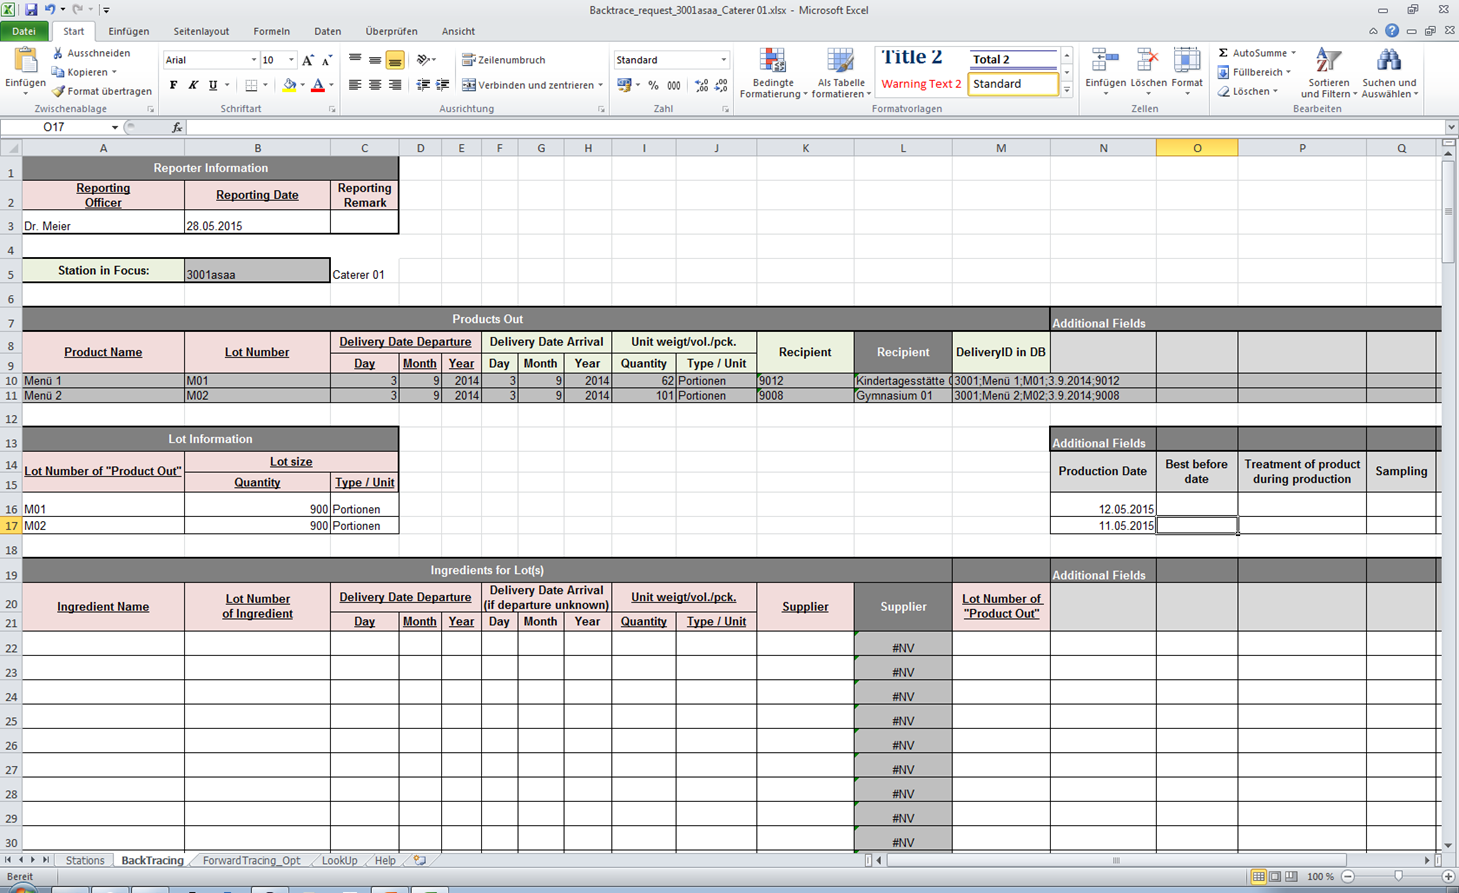
\includegraphics[height=0.6\textheight]{14.png}
	\end{center}
	\begin{itemize}
		\item In unserem Fall waren die Information \textbf{Lot size} bereits vorhanden, so daß hier keine Informationen eingetragen werden müssen. Sollten hier falsche Zahlen stehen müssen sie korrigiert werden.
		\item Es besteht die Möglichkeit eigene \textbf{Additional Fields} zu definieren und Daten dazu erfassen, hier im Beispiel für \textbf{Production Date}.
	\end{itemize}
\end{frame}

\section{15}
\begin{frame}
	\begin{center}
  		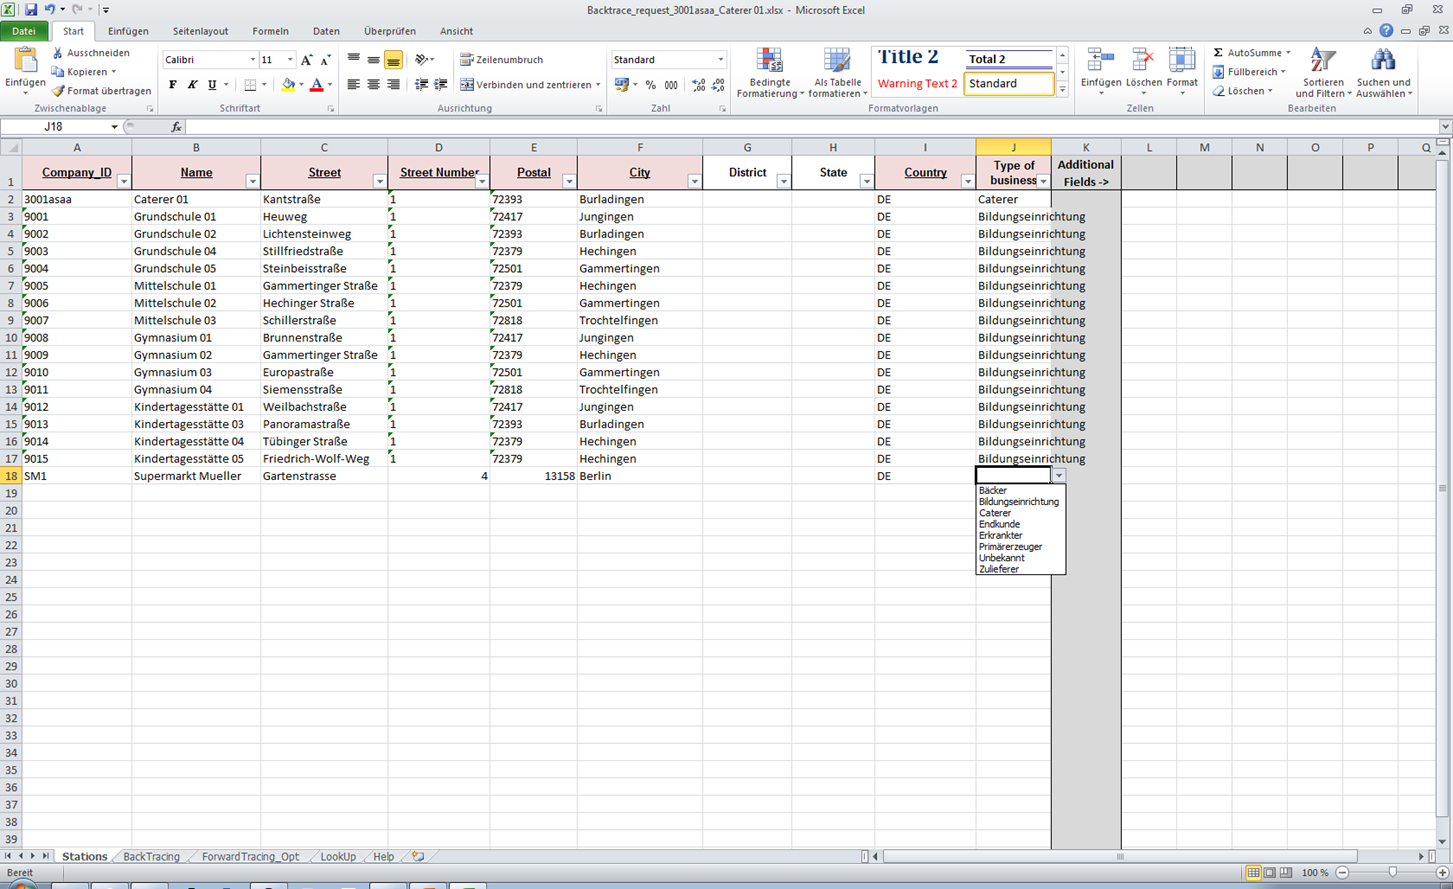
\includegraphics[height=0.6\textheight]{15.png}
	\end{center}
	\begin{itemize}
		\item Im Tabellenblatt \textbf{Stations} können neue Stationen angelegt werden.
		\item Legen Sie hier die neue Station \textbf{Supermarkt Mueller} an.
		\item Geben Sie der neuen Station den \textbf{Type of business} '\textbf{Zulieferer}'.
	\end{itemize}
\end{frame}

\section{16}
\begin{frame}
	\begin{center}
  		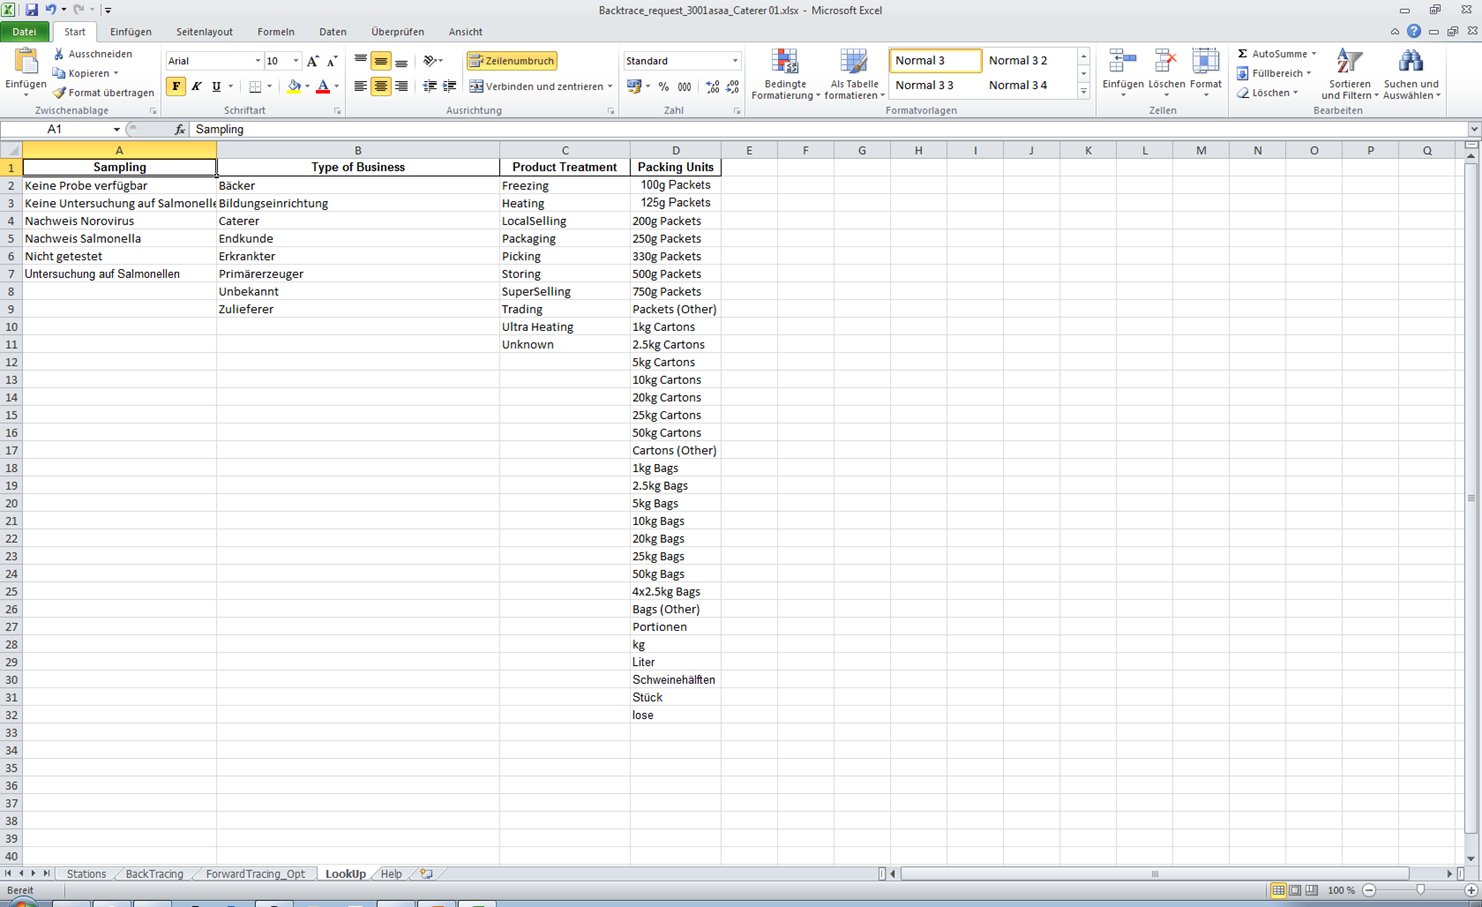
\includegraphics[height=0.6\textheight]{16.png}
	\end{center}
	\begin{itemize}
		\item Die Auswahlmöglichkeiten mehrerer Auswahlfelder wie z.B. für \textbf{Type of business} sind im Tabellenblatt \textbf{LookUp} definiert.
		\item Dort können neue LookUps angelegt oder korrigiert werden.
		\item Optimalerweise werden Änderungen hierin mit dem zentralen Datenmanager abgesprochen.
	\end{itemize}
\end{frame}

\section{17}
\begin{frame}
	\begin{center}
  		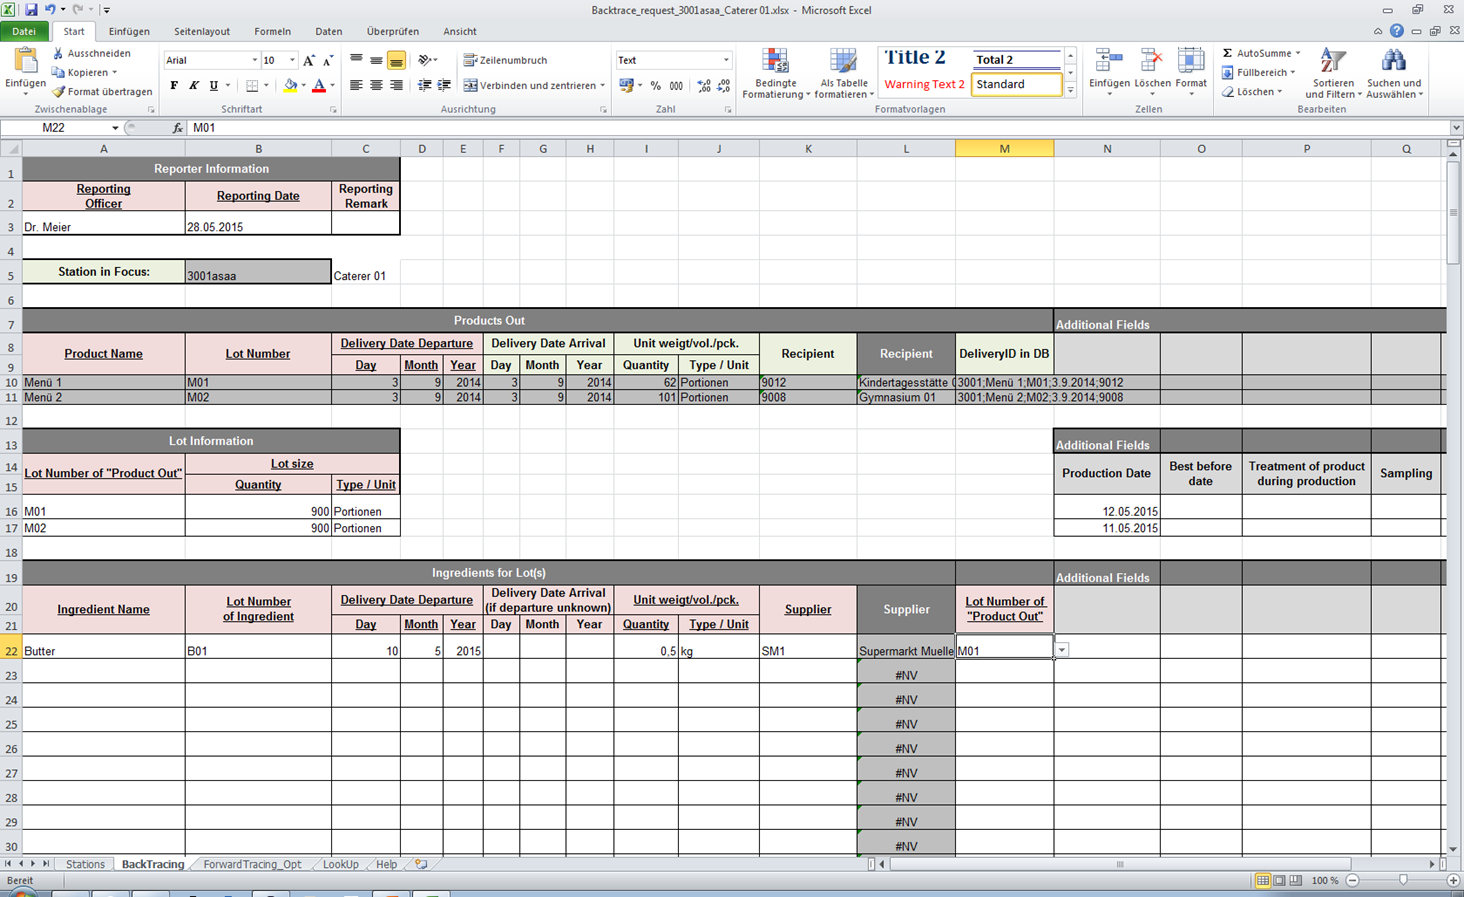
\includegraphics[height=0.6\textheight]{17.png}
	\end{center}
	\begin{itemize}
		\item Im Tabellenblatt \textbf{BackTracing} definieren Sie nun die Zutaten zu den beiden vorgegebenen Lieferungen bzw. Lots.
		\item Dazu füllen Sie die Zeilen ab Zeile 22 aus.
	\end{itemize}
\end{frame}

\section{18}
\begin{frame}
	\begin{center}
  		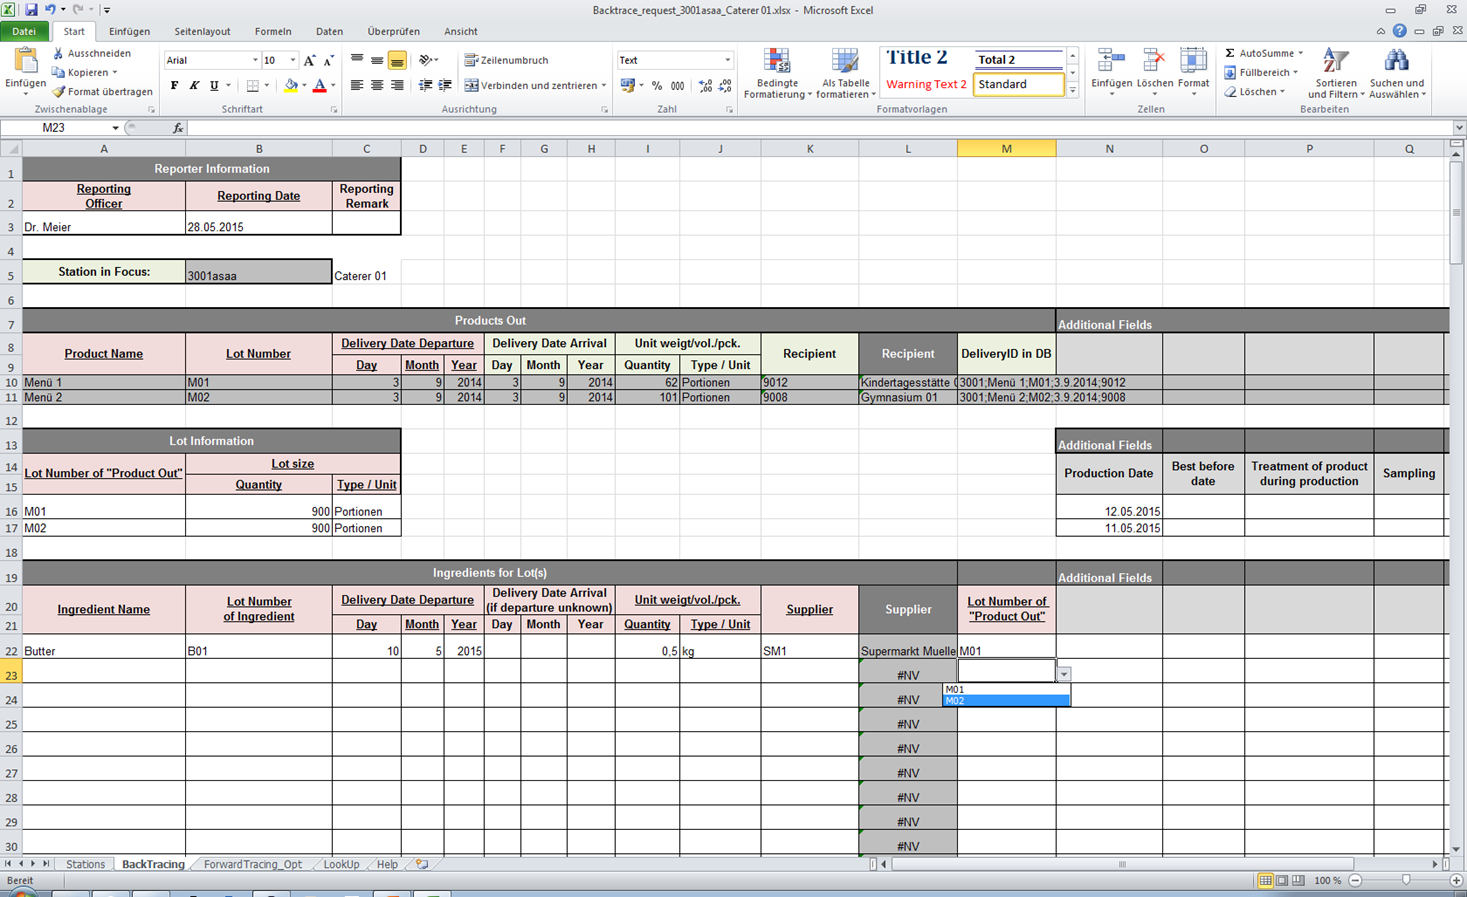
\includegraphics[height=0.6\textheight]{18.png}
	\end{center}
	\begin{itemize}
		\item Achten Sie darauf zu jeder eingetragenen Lieferung die zugehörige Lotnummer auszuwählen (Spalte M).
	\end{itemize}
\end{frame}

\section{19}
\begin{frame}
	\begin{center}
  		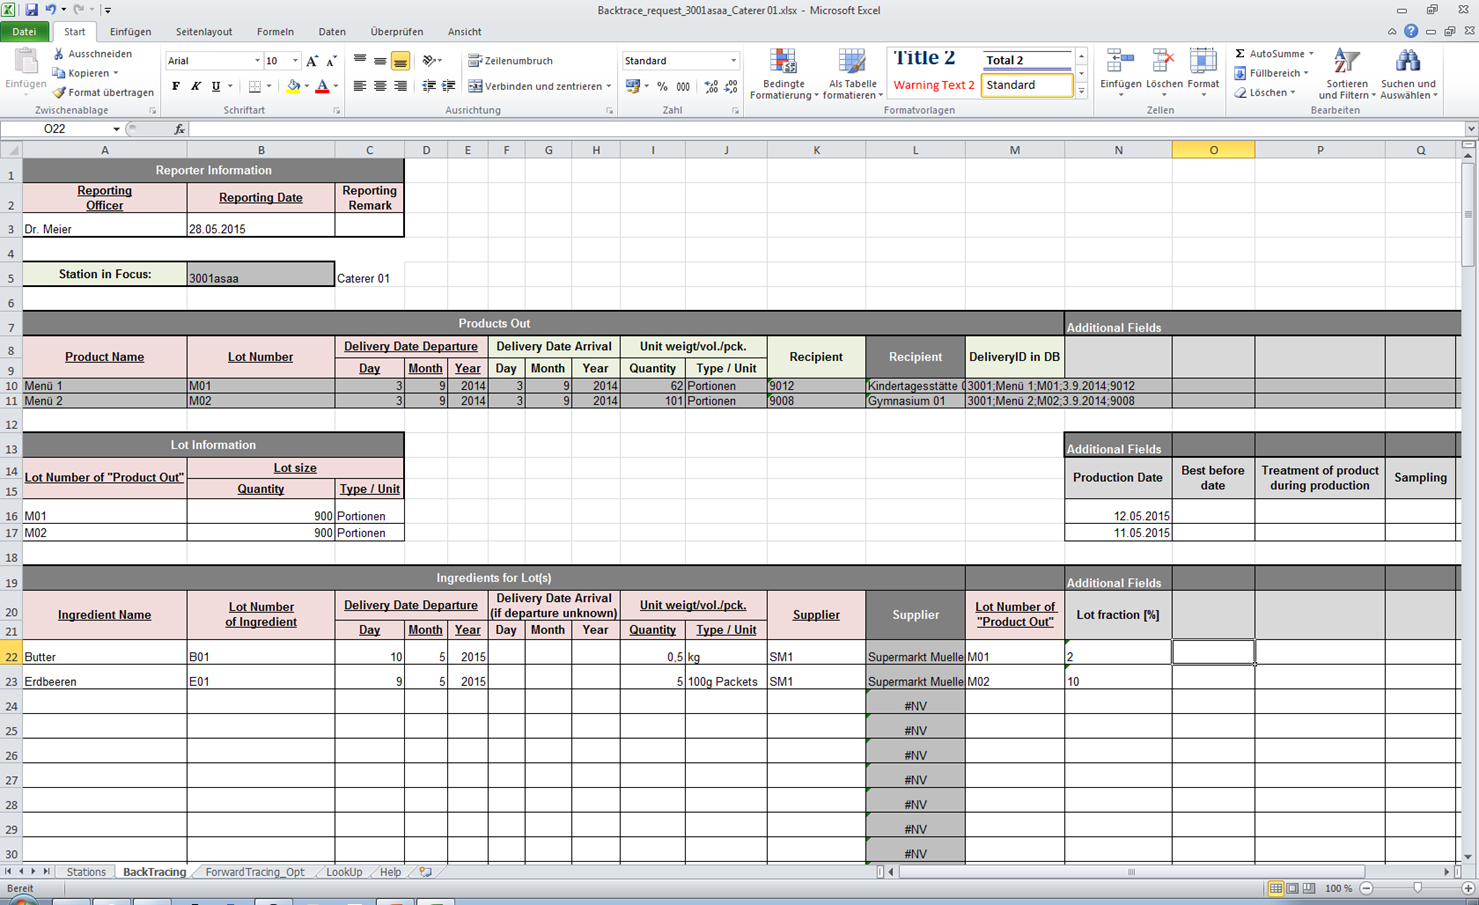
\includegraphics[height=0.6\textheight]{19.png}
	\end{center}
	\begin{itemize}
		\item Auch hier ist es möglich \textbf{Additional Fields} zu definieren und Daten dazu erfassen, hier im Beispiel für \textbf{Lot fraction [\%]}.
		\item Diese definierten Felder sind dann für die Analyse genauso verfügbar.
		\item Normalerweise gibt der Datenmanager vor, welche Felder zusätzlich ausgefüllt werden sollen.
	\end{itemize}
\end{frame}

\section{20}
\begin{frame}
	\begin{center}
  		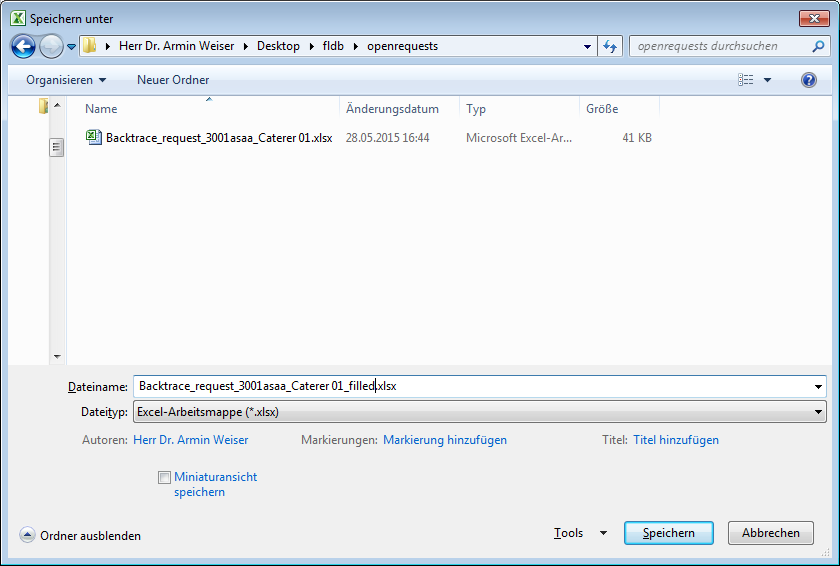
\includegraphics[height=0.6\textheight]{20.png}
	\end{center}
	\begin{itemize}
		\item Speichern Sie das ausgefüllte Template und merken Sie sich den Ordner, in dem Sie es abgespeichert haben.
	\end{itemize}
\end{frame}


\section{21}
\begin{frame}
	\begin{center}
  		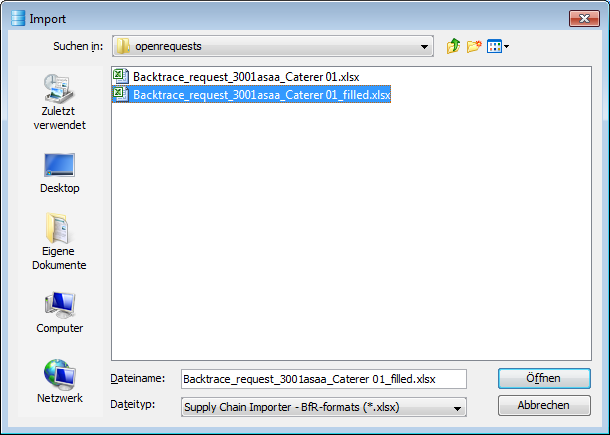
\includegraphics[height=0.6\textheight]{21.png}
	\end{center}
	\begin{itemize}
		\item Wechseln Sie wieder zu dem Datenbankfenster, ggf. öffnen Sie es wieder via \textbf{Food-Lab $>$ Open DB Gui...}.
		\item Drücken Sie auf das Ordnersymbol mit dem blauen Pfeil.
		\item Dadurch öffnet sich der Importdialog.
		\item Wählen Sie im Importdialog die Exceldatei aus, die Sie soeben abgespeichert haben.
		\item Klicken Sie auf \textbf{Öffnen}.
	\end{itemize}
\end{frame}

\section{22}
\begin{frame}
	\begin{center}
  		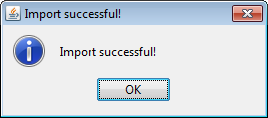
\includegraphics[height=0.3\textheight]{22.png}
	\end{center}
	\begin{itemize}
		\item Die Tabellen der Datenbank haben sich weiter gefüllt.
		\item Der erfolgreiche Import wird durch ein kleines Fenster  bekanntgegeben.
		\item Schließen Sie dieses Fenster durch Klicken auf \textbf{OK}.
		\item Sie können die Daten jetzt mit FoodChain-Lab analysieren. Schauen Sie dazu bei Bedarf in die entsprechenden Tutorials.
	\end{itemize}
\end{frame}

\end{document}